% ------------------------------------------------------------------------------
% TYPO3 CMS 7.6 - What's New - Chapter "Introduction" (English Version)
%
% @author	Michael Schams <schams.net>
% @license	Creative Commons BY-NC-SA 3.0
% @link		http://typo3.org/download/release-notes/whats-new/
% @language	English
% ------------------------------------------------------------------------------
% LTXE-CHAPTER-UID:		cb43d098-7bf9a537-bf3817c0-53a0f29f
% LTXE-CHAPTER-NAME:	Introduction
% ------------------------------------------------------------------------------

\section{Introducción}
\begin{frame}[fragile]
	\frametitle{Introducción}

	\begin{center}\huge{Introducción}\end{center}
	\begin{center}\huge{\color{typo3darkgrey}\textbf{Los Hechos}}\end{center}

\end{frame}

% ------------------------------------------------------------------------------
% LTXE-SLIDE-START
% LTXE-SLIDE-UID:		680cf77c-a20d02ae-2231eced-bf57562c
% LTXE-SLIDE-ORIGIN:	9e397afb-762f7061-0e0e0bd1-9836250e English
% LTXE-SLIDE-ORIGIN:	1e50fa0a-e0f4c00a-5f667356-11df7c7c German
% LTXE-SLIDE-TITLE:		TYPO3 CMS 7.6 - The Facts
% ------------------------------------------------------------------------------
\begin{frame}[fragile]
	\frametitle{Introducción}
	\framesubtitle{TYPO3 CMS 7.6 - Los Hechos}

	\begin{itemize}
		\item Fecha de lanzamiento: 10 Noviembre 2015
		\item Tipo de lanzamiento:
			\begingroup\color{red}Lanzamiento Soporte a Largo Plazo (LTS)\endgroup
		\item Visión: Adoptar, Innovar, Lanzar
	\end{itemize}

	\begin{figure}
		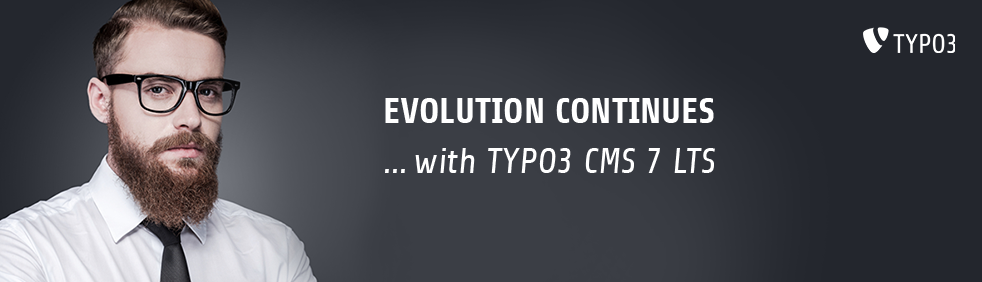
\includegraphics[width=0.95\linewidth]{Introduction/typo3cms76-banner.png}
	\end{figure}

\end{frame}

% ------------------------------------------------------------------------------
% LTXE-SLIDE-START
% LTXE-SLIDE-UID:		3bddf583-8e0ca258-614420f9-13337323
% LTXE-SLIDE-ORIGIN:	737c8e9b-4ae60e26-6975ea72-21146dd0 English
% LTXE-SLIDE-ORIGIN:	07f94e22-95cf3db6-373b81e0-4b00bb57 German
% LTXE-SLIDE-TITLE:		System Requirements
% ------------------------------------------------------------------------------
\begin{frame}[fragile]
	\frametitle{Introducción}
	\framesubtitle{Requisitos del Sistema}

	\begin{itemize}
		\item PHP*:\tabto{2.2cm}v5.5.0 - v5.6.x
		\item MySQL:\tabto{2.2cm}v5.5.x - v5.6.x (modo no estricto)
		\item Espacio de disco:\tabto{2.2cm}min 200 MB
		\item Ajustes de PHP:

			\begin{itemize}
				\item memory\_limit >= 128M
				\item max\_execution\_time >= 240s
				\item opción de compilación \texttt{--disable-ipv6} \underline{no} debe ser usada
			\end{itemize}

		\item Backend requiere IE >= 9 o cualquier otro navegador moderno

	\end{itemize}

	\vspace{1cm}

	*) Detalles adicionales: \href{http://typo3.org/news/article/php-minimum-requirements-for-typo3-cms-7/}{Requisitos Mínimos de PHP para TYPO3 CMS 7}

\end{frame}

% ------------------------------------------------------------------------------
% LTXE-SLIDE-START
% LTXE-SLIDE-UID:		0488974b-40c53045-51b5b5a5-cdcf450d
% LTXE-SLIDE-ORIGIN:	90d2d3d1-f9d57661-dd01143b-10630416 English
% LTXE-SLIDE-ORIGIN:	79b3ee12-a96f5128-178eb0a1-52534b81 German
% LTXE-SLIDE-TITLE:		Development And Release Timeline
% ------------------------------------------------------------------------------
\begin{frame}[fragile]
	\frametitle{Introducción}
	\framesubtitle{Línea de tiempo de Desarrollo y Lanzamiento}

	\begin{figure}
		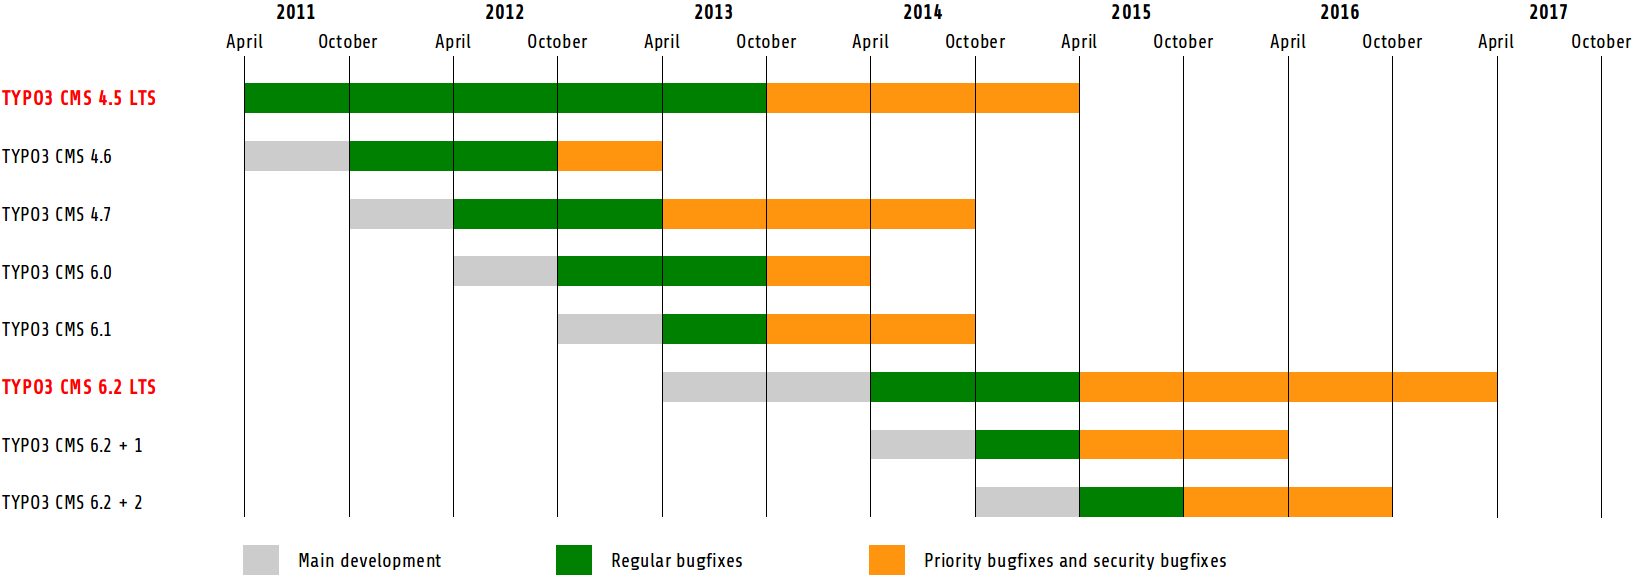
\includegraphics[width=0.90\linewidth]{Introduction/ReleaseAgenda.png}
	\end{figure}

\end{frame}

% ------------------------------------------------------------------------------
% LTXE-SLIDE-START
% LTXE-SLIDE-UID:		cef12282-a0e48424-22722f3f-47b9f8a2
% LTXE-SLIDE-ORIGIN:	13e0fd6a-fa50d02d-c15c4af0-f3996926 English
% LTXE-SLIDE-ORIGIN:	89509115-eb2b6501-4bf03801-c53e7c0c German
% LTXE-SLIDE-TITLE:		TYPO3 CMS Roadmap
% ------------------------------------------------------------------------------
\begin{frame}[fragile]
	\frametitle{Introducción}
	\framesubtitle{Línea de lanzamiento de TYPO3 CMS}

	Fechas de lanzamiento estimadas y sus enfoques principales:

	\begin{itemize}
		\item v7.0 \tabto{1.1cm}02/Dez/2014\tabto{3.4cm}Revisión de Backend Vol 1
		\item v7.1 \tabto{1.1cm}24/Feb/2015\tabto{3.4cm}Optimización \& Limpieza del núcleo
		\item v7.2 \tabto{1.1cm}28/Apr/2015\tabto{3.4cm}Frontend
		\item v7.3 \tabto{1.1cm}16/Jun/2015\tabto{3.4cm}Ecosistema de Paquetes, Composer
		\item v7.4 \tabto{1.1cm}04/Aug/2015\tabto{3.4cm}Revisión de Backend Vol 2
		\item v7.5 \tabto{1.1cm}29/Sep/2015\tabto{3.4cm}Finalización

		\item
			\begingroup
				\color{typo3orange}
					v7 LTS \tabto{1.1cm}10/Nov/2015\tabto{3.4cm}\textbf{TYPO3 CMS 7 LTS} (Soporte a Largo Plazo)
			\endgroup

	\end{itemize}

	\smaller
		\url{https://typo3.org/typo3-cms/roadmap/}\newline
		\url{http://typo3.org/news/article/embrace-and-innovate-typo3-cms-7/}
	\normalsize

\end{frame}

% ------------------------------------------------------------------------------
% LTXE-SLIDE-START
% LTXE-SLIDE-UID:		31722c57-0d4c9a90-728417eb-ec4af01b
% LTXE-SLIDE-ORIGIN:	06c6100a-69216610-618bde63-bbdc4eef English
% LTXE-SLIDE-ORIGIN:	8ac7908b-f1a64895-d12d437b-9309b07b German
% LTXE-SLIDE-TITLE:		Installation
% ------------------------------------------------------------------------------
\begin{frame}[fragile]
	\frametitle{Introducción}
	\framesubtitle{Instalación}

	\begin{itemize}
		\item Procedimiento de instalación oficial bajo Linux/Mac OS X\newline
			(DocumentRoot por ejemplo \texttt{/var/www/site/htdocs}):
		\begin{lstlisting}
			$ cd /var/www/site
			$ wget --content-disposition get.typo3.org/7.6
			$ tar xzf typo3_src-7.6.0.tar.gz
			$ cd htdocs
			$ ln -s ../typo3_src-7.6.0 typo3_src
			$ ln -s typo3_src/index.php
			$ ln -s typo3_src/typo3
			$ touch FIRST_INSTALL
		\end{lstlisting}

		\item Enlaces simbólicos bajo Microsoft Windows:

			\begin{itemize}
				\item Use \texttt{junction} en Windows XP/2000
				\item Use \texttt{mklink} en Windows Vista y Windows 7
			\end{itemize}

	\end{itemize}
\end{frame}

% ------------------------------------------------------------------------------
% LTXE-SLIDE-START
% LTXE-SLIDE-UID:		aea93dea-066e7968-7cf47d1b-059b5764
% LTXE-SLIDE-ORIGIN:	e4b09ddf-4c0ea575-9e0900ad-b878899c English
% LTXE-SLIDE-ORIGIN:	d146f854-4fcfed01-7de68fce-c2599f7f German
% LTXE-SLIDE-TITLE:		Upgrade to TYPO3 CMS 7
% ------------------------------------------------------------------------------
\begin{frame}[fragile]
	\frametitle{Introducción}
	\framesubtitle{Actualización a TYPO3 CMS 7.x}

	\begin{itemize}
		\item Actualizaciones sólo posibles desde TYPO3 CMS 6.2 LTS
		\item TYPO3 CMS < 6.2 debe ser actualizado a TYPO3 CMS 6.2 LTS primero
	\end{itemize}

	\begin{itemize}

		\item Instrucciones de actualización:\newline
			\smaller\url{http://wiki.typo3.org/Upgrade#Upgrading_to_7.6}\normalsize
		\item Guía oficial de TYPO3 "Instalación y Actualización de TYPO3":
			\smaller\url{http://docs.typo3.org/typo3cms/InstallationGuide}\normalsize
		\item Enfoque general:
			\begin{itemize}
				\item Comprobar requisitos mínimos del sistema \small(PHP, MySQL, etc.)
				\item Revisar \textbf{deprecation\_*.log} en instancia antigua de TYPO3
				\item Actualizar todas las extensiones a la última versión
				\item Desplegar fuentes nuevas y ejecutar Herramienta de Instalación \textrightarrow Asistente de Actualización
				\item Revisar el módulo de inicio para usuarios backend (opcionalmente)
			\end{itemize}
	\end{itemize}

\end{frame}

% ------------------------------------------------------------------------------
